\chapter{Reconstruction of the $t\bar{t}$ Kinematics}\label{chapt:kinReco}

The two neutrinos are not detected, thus additional
assumptions are needed to define the full final state kinematics of the $t\bar{t}$ reconstructed in dilepton decay channel.
This section describes a method used for the full kinematics reconstruction of this system. A mathematical
background (sec. \ref{sec:MatBg}) as well as a performance description of the method (sec. \ref{sec:SolSer} -- \ref{sec:kinRecPerf}) are revealed.

\section{Mathematical Background}\label{sec:MatBg}

The presence of two undetected neutrinos introduces six unknowns  (three momentum components of each neutrino)
to the $t\bar{t}$ system in the dilepton final state.
The following constrains are being used:

\begin{itemize}
 \item \textit{t and $\bar{t}$ masses} ($m_{t}$ and $m_ {\bar{t}}$) are assumed to be equal and constrained to the same value of 172.5 GeV\cite{PDG-2012};
 \item The whole missing transverse energy $E_{T}^{miss}$ of the event is assumed to arise entirely
 from the two neutrinos from the $t\bar{t}$ decay;
 \item \textit{The $W^{\pm}$ masses} ($m_{W\pm}$) are assumed to be known and constrained to the value which is randomly taken
 from the generator $W^{\pm}$ mass spectrum.
\end{itemize}

These assumptions lead to the system of six equations which describe energies and momenta conservation:

\begin{align}\label{alg:LS1}
 E^{miss}_{T_{x}} & =  p_{\nu_{x}} + p_{\bar{\nu}_{x}} \\
 %
 E^{miss}_{T_{y}} & =  p_{\nu_{y}} + p_{\bar{\nu}_{y}} \\
 %
 m^{2}_{W^{+}} & = (E_{l^{+}} + E_{\nu})^{2} - (p_{l^{+}_{x}} + p_{\nu_{x}})^{2} - (p_{l^{+}_{y}} + p_{\nu_{y}})^{2} - (p_{l^{+}_{z}} + p_{\nu_{z}})^2 \\
 %
 m^{2}_{W^{-}} & = (E_{l^{-}} + E_{\bar{\nu}})^{2} - (p_{l^{-}_{x}} + p_{\bar{\nu}_{x}})^{2} - (p_{l^{-}_{y}} + p_{\bar{\nu}_{y}})^{2} - (p_{l^{-}_{z}} + p_{\bar{\nu}_{z}})^2 \\
 % 
 m_{t}^{2} & = (E_{b} + E_{l^{+}} + E_{\nu})^{2} - (p_{b_{x}} + p_{l^{+}_{x}} + p_{\nu_{x}})^2 \nonumber \\
           & - (p_{b_{y}} + p_{l^{+}_{y}} + p_{\nu_{y}})^2 - (p_{b_{z}} + p_{l^{+}_{z}} + p_{\nu_{z}})^2 \\
 %
 m_{\bar{t}}^{2} & = (E_{\bar{b}} + E_{l^{-}} + E_{\bar{\nu}})^{2} - (p_{\bar{b}_{x}} + p_{l^{-}_{x}} + p_{\bar{\nu}_{x}})^2 \nonumber \\
                 & - (p_{\bar{b}_{y}} + p_{l^{-}_{y}} + p_{\bar{\nu}_{y}})^2 - (p_{\bar{b}_{z}} + p_{l^{-}_{z}} + p_{\bar{\nu}_{z}})^2\label{alg:LS6} 
\end{align}

Here the $E_{l^{\pm}}$ and $p_{l^{\pm}_{x,y,z}}$ correspond to the lepton(antilepton) energy and momentum components respectively; 
$E_{b/\bar{b}}$ and $p_{b/\bar{b}_{x,y,z}}$ are the $b$/$\bar{b}$-jet energy and momentum components respectively; the $E^{miss}_{T_{x,y}}$ are
the two components of the missing transverse energy; the $p_{\nu/\bar{\nu}_{x,y,z}}$ are the neutrino (antineutrino) momenta components.
The neutrino energies $ E_{\nu/\bar{\nu}}$ are composed from momenta:

\begin{equation}
 E_{\nu/\bar{\nu}}^{2} = p_{\nu/\bar{\nu}_{x}}^{2} + p_{\nu/\bar{\nu}_{y}}^{2} + p_{\nu/\bar{\nu}_{z}}^{2}
\end{equation}

$E_{l^{\pm}}$, $p_{l^{\pm}_{x,y,z}}$, $E_{b/\bar{b}}$, $p_{b/\bar{b}_{x,y,z}}$ and $E^{miss}_{T_{x,y}}$ are reconstructed from the detector (as described in the chapter \ref{chapt:event_selection})
and $p_{\nu/\bar{\nu}_{x,y,z}}$ are the unknowns.

The analytical solution of the system of equations (\ref{alg:LS1}--\ref{alg:LS6}) was proposed in \cite{LSpaper}. After a number of transformations
the system is reduced to the fourth order polynomial equation of a neutrino momentum component $p_{\nu_{x}}$:

\begin{equation}\label{eq:eqLSf}
 0 = h_{0} p_{\nu_{x}}^{4} + h_{1} p_{\nu_{x}}^{3} + h_{2} p_{\nu_{x}}^{2} + h_{3} p_{\nu_{x}} + h_{4},
\end{equation}

where the coefficients $h_{0} - h_{4}$ \cite{LSpaper, LSerrat} depend on the missing transverse energy $E_{T}^{miss}$ and four-momenta of the
leptons and jets. 

The equation \ref{eq:eqLSf} ends up with up to four solutions. The frequency distribution of the number of solutions for generated $t\bar{t}$ sample (MadGraph+Pythia,
see chapt. \ref{chapt:MC}) is shown on the Figure \ref{fig:LSNsol}. Two solutions per event are expected in 80$\%$ of the cases and four solutions per event appear in 
$20\%$ of the cases.

\begin{figure}[t]
  \centering
  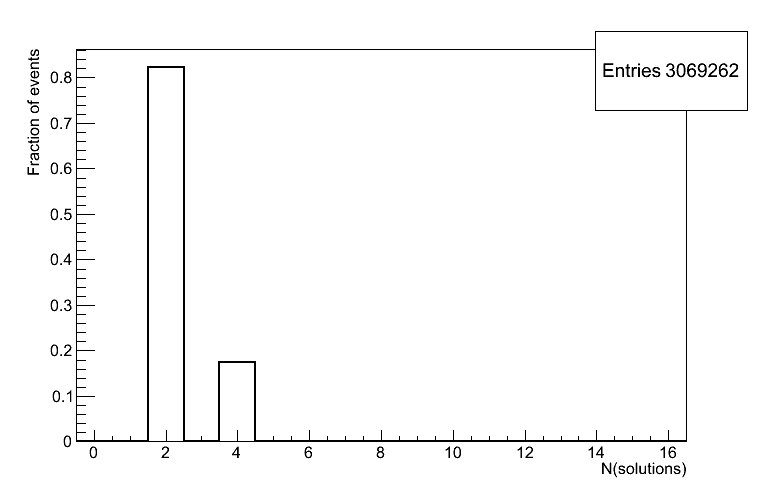
\includegraphics[width=0.8\textwidth]{05_kinReco/plots/KinReco_Nsolutions.png}
  \caption{Number of solutions of the equation \ref{eq:eqLSf}. The distribution is normalized to one. The information used for this plot is taken
  from the generator level MC used for this analysis.}
  \label{fig:LSNsol}
\end{figure}


% Under the real conditions a sizable amount of the events will find no solutions of the kinematic equations (\ref{alg:LS1}--\ref{alg:LS6})
% because of an imperfect reconstruction of the detector objects. But in the other cases there is a possibility to find up to four solutions.

\section{Ambiguity and Detector Effects Treatment}\label{sec:SolSer}

There are several problems arising during the $t\bar{t}$ dilepton final state kinematics reconstruction:

\begin{itemize}
 \item \textit{Fluctuations of measurement}. There might be no solutions found for a combination
 of leptons, jets and missing transverse energy arising from the $t\bar{t}$ system due to reconstruction effects, e.g. detector resolution,
 jet finder inaccuracy, badly reconstructed missing transverse energy, etc.
 %
 \item \textit{Multiple solutions of the kinematic equations}. As discussed in section \ref{sec:MatBg} the solution of the equation \ref{eq:eqLSf}
 provides up to four correct solutions while a real neutrino has only one momentum.
 %
 \item \textit{Multiple combinations of leptons and jets}. An event with a $t\bar{t}$ decaying to a dilepton final state has minimum two leptons and two
 jets. However there is no sign if a jet comes from $t$ or a $\bar{t}$. For this reason each jet is being paired to one of the leptons, and then to another
 to form a $t$ or $\bar{t}$ candidate. Thus an event with two leptons and two jets has two possible $t\bar{t}$ candidates. In case of multiple jets
 in the event, the number of $t\bar{t}$ candidates can be up to $N_{jet}!$, where $N_{jet}$ is a jet multiplicity.
\end{itemize}

% The last two challenges have different nature but boths cause the same issue of multiple possible $t\bar{t}$ candidates, thus they can be treated together.

\subsection{Fluctuations of measurements}

The problem of rescuing the events which are lost due to the fluctuations is solved by varying the measured objects energies and
momentum directions. That will increase the efficiency of finding a solution of the system of equations (\ref{alg:LS1}--\ref{alg:LS6}). The idea was implemented by reconstructing
each event 100 times, each time varying relevant observables according to their resolution determined from the Monte Carlo.
The leptons and jets energies and directions were smeared. All the variations are done randomly, independently and simultaneously for every quantity.

The energy variation was performed through multiplication of an actual reconstructed energy value
by a correction factor $f(E) = \frac{E_{true}}{E_{reco}}$. Here the $E_{reco}$ is the reconstructed lepton or jet energy taken from the MC signal simulation;
the $E_{true}$ is the true energy of the same object on the particle level. The distributions for the $f(E)$ which are used for the random choice
of the correction factors are shown on the Figure \ref{fig:fE}. The correction factors which enter the distributions are determined from the signal MC simulation jets and 
leptons matched to the particle level $b$-quarks and leptons arising from the top decay. 

\begin{figure}[t]
\centering
\begin{subfigure}
  \centering
  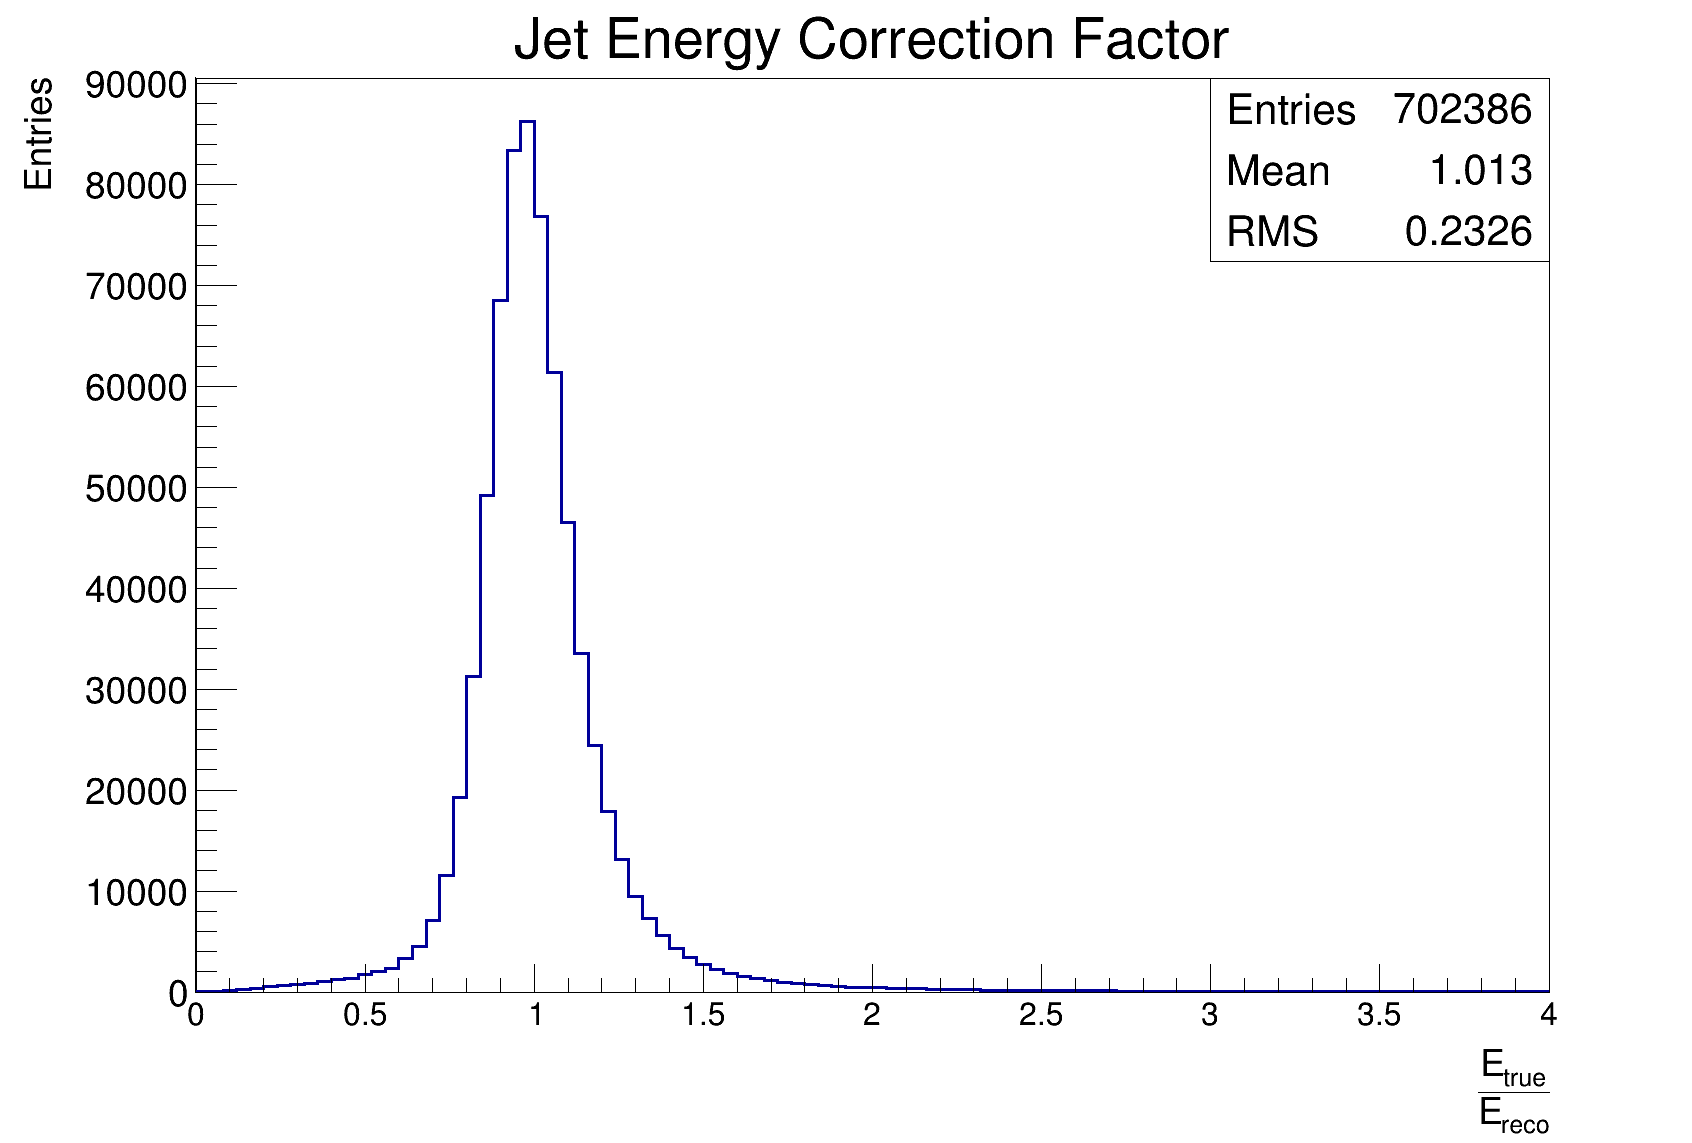
\includegraphics[width=0.48\textwidth]{05_kinReco/plots/fE_jet.png}
\end{subfigure}
\begin{subfigure}
  \centering
  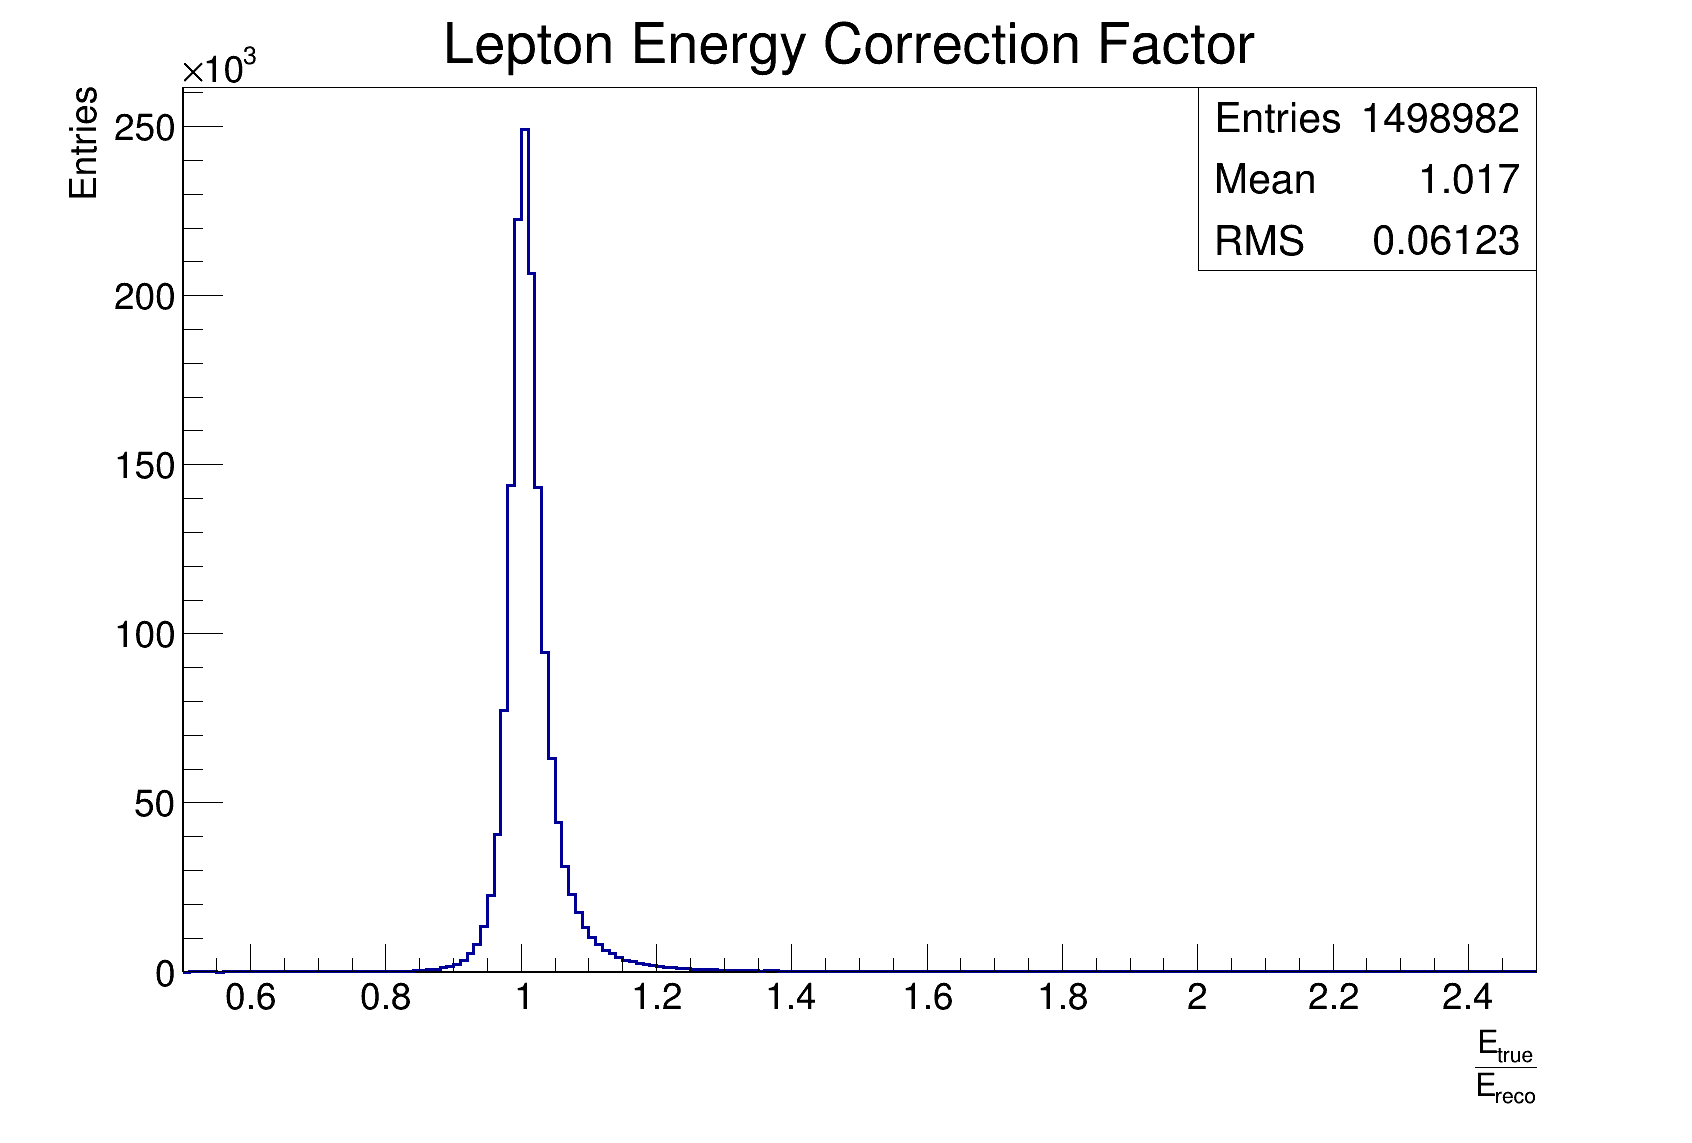
\includegraphics[width=0.48\textwidth]{05_kinReco/plots/fE_lep.png}
\end{subfigure}
\caption{Distributions of the energy correction factors used for the energy smearing in the kinematic
reconstruction of the top-quark kinematics. The factor distribution for jets is shown on the left and for
the leptons -- on the right.}
\label{fig:fE}
\end{figure}

Directional smearing is applied by varying the azimuth and polar angles (see sec. \ref{sec:CMS}). A smearing of the azimuth angle $\theta$ is performed in a random direction taken from
the MC distributions presented on the Figure \ref{fig:dAngle}. The polar angle $\phi$ is taken randomly from 0 to $2\pi$.

\begin{figure}[t]
\centering
\begin{subfigure}
  \centering
  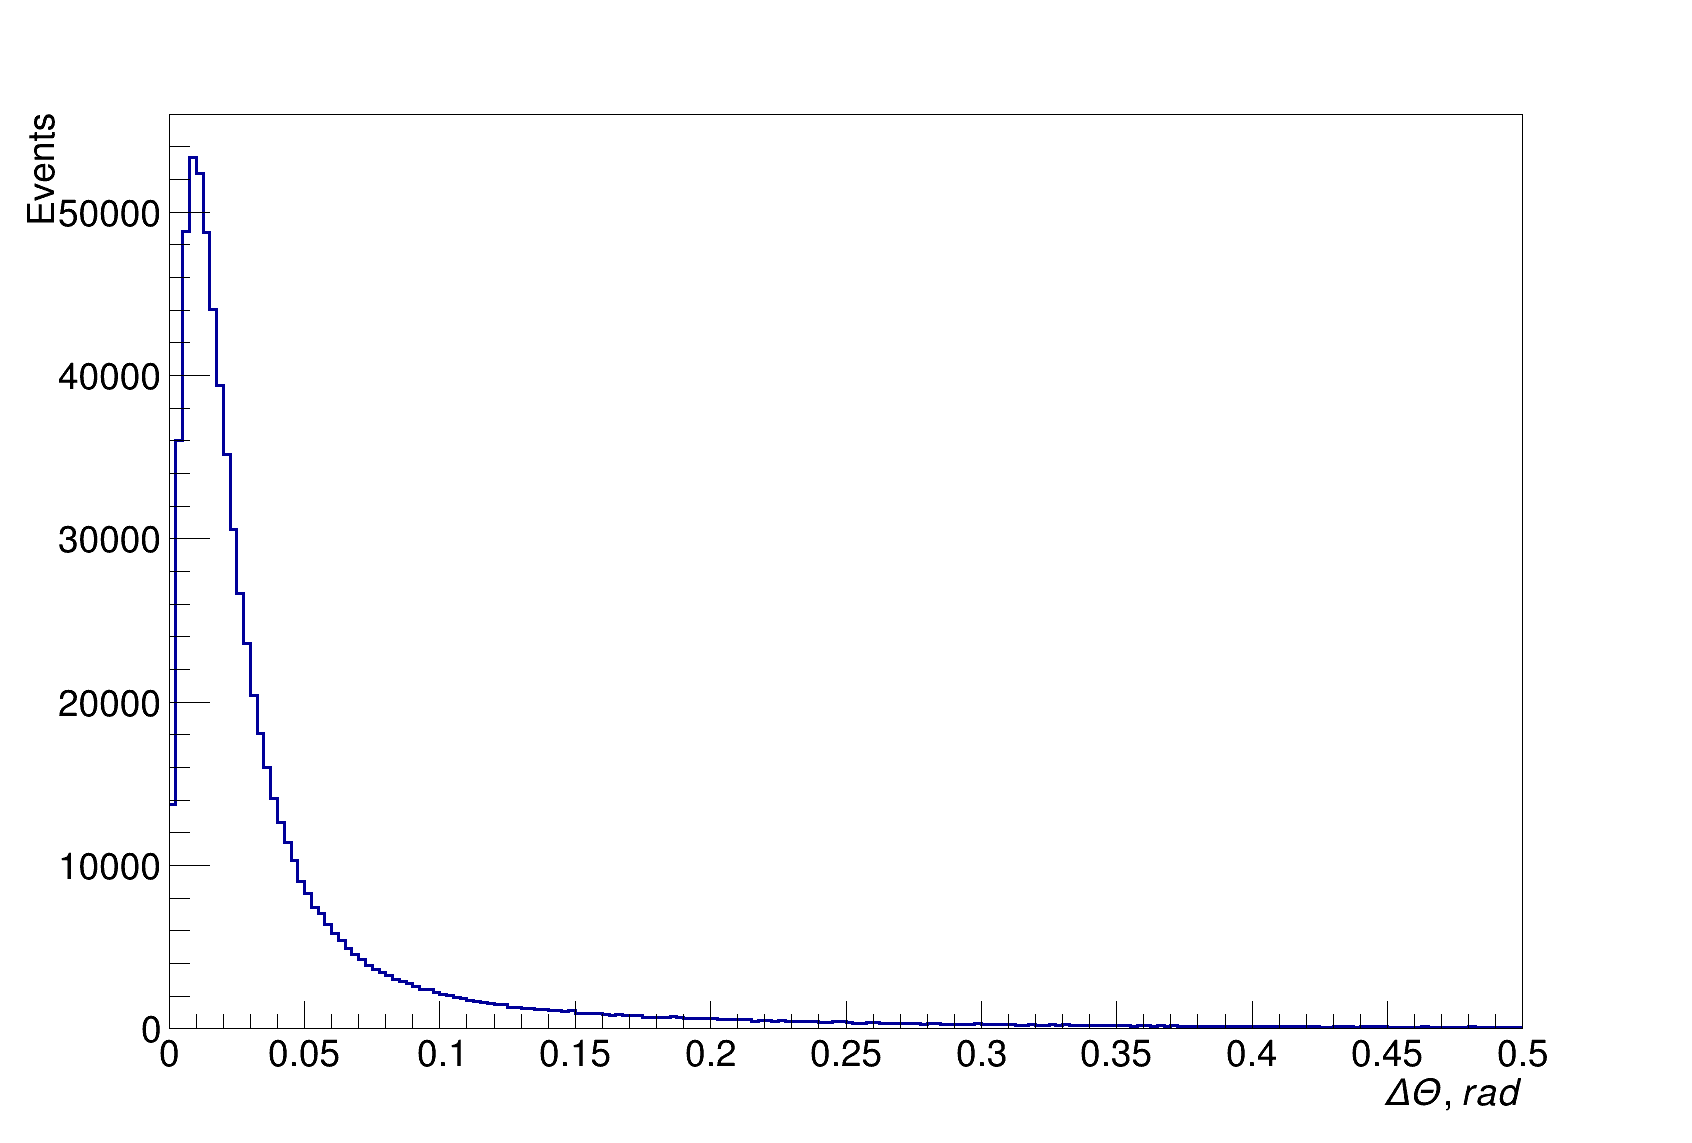
\includegraphics[width=0.48\textwidth]{05_kinReco/plots/dan_jet.png}
\end{subfigure}
\begin{subfigure}
  \centering
  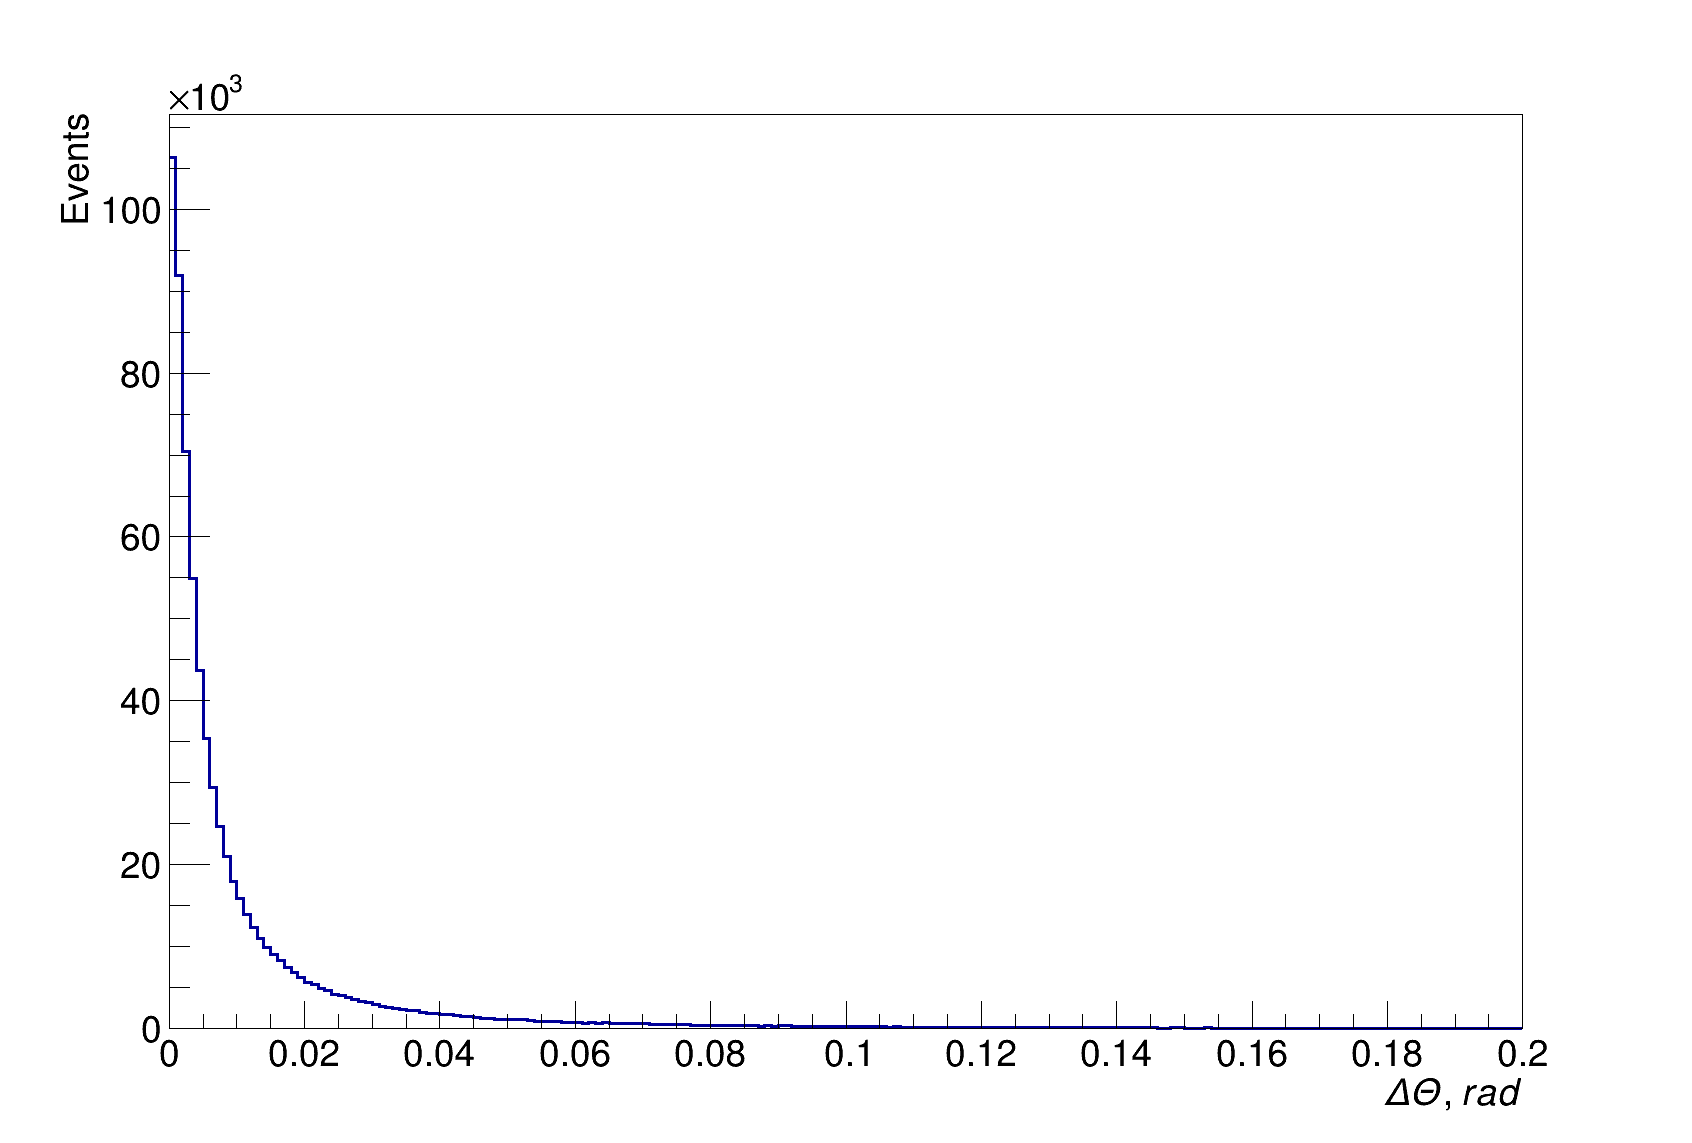
\includegraphics[width=0.48\textwidth]{05_kinReco/plots/dan_lep.png}
\end{subfigure}
\caption{Distributions of the angle between the particle level direction and the detector level direction.
The angle distribution for the b quarks is shown on the left and for the leptons -- on the right.}
\label{fig:dAngle}
\end{figure}

In each of the 100 jet and lepton kinematics variations the transverse missing energy $E_{T}^{miss}$ has to be recalculated. This is done
assuming the transverse energy component, which does not refer to the leptons and jets forming a $t\bar{t}$ candidate, to be constant. Thus,
missing transverse energy for the $i^{th}$ smearing will be expressed as following:

\begin{equation}
 E^{miss\;i}_{T_{x,y}} = E^{miss \; from \, reconstruction}_{T_{x,y}} + p^{jet \; not\,smeared}_{x,y} + p^{lepton\;not\,smeared}_{x,y} - (p^{jet\;i}_{x,y} + p^{lepton\;i}_{x,y})
\end{equation}

\subsection{Single solution choice}

The equation \ref{eq:eqLSf} is solved for every of the 100 event reconstructions. Each equation may have up to four solutions, thus each event
has up to ($100 \otimes 4 \otimes N_{jet}!$) reconstructed $t\bar{t}$ candidates ($N_{jet}!$ component has already been discussed is sec. \ref{sec:SolSer}). 
To obtain one $t\bar{t}$ pair out of this candidate variety, following steps are undertaken:

\begin{itemize}
 \item [--] For each of the four solutions of the equation \ref{eq:eqLSf} the invariant of the $t\bar{t}$ pair, $m(t\bar{t})$, is calculated. Only
 the solution which has the smallest $m(t\bar{t})$ is taken. This criterion was prior introduced in \cite{PhysRevD.73.112006}, where it was shown to
 deliver for the correct lepton-jet assignment in most cases the correct solution.
 %
 \item [--] To the rest of up to ($100 \otimes N_{jet}!$) candidates a weight $\omega = \omega_{m^{\bar{l}b}} \dot \omega_{m^{l\bar{b}}}$
 is calculated. Here $m^{\bar{l}b}$ and $m^{l\bar{b}}$ are the reconstructed invariant masses of the lepton-jet pairs from the top and the anti-top 
 decays, respectively. These weights are calculated from the spectrum of the lepton-jet pairs in top decays obtained from a signal MC on the 
 particle level after all kinematic cuts described in chapter \ref{chapt:event_selection}. A $t$ ($\bar{t}$) momentum is constructed as a wighted 
 average of all smeared solutions as following:
 \begin{equation}
  \langle{\vec{p}(t,\bar{t})}\rangle = \frac{\sum\limits_{i=1}^{100} \omega_{i} \vec{p(t,\bar{t})}_i}{\sum\limits_{i=1}^{100} \omega_i}.
 \end{equation}
 Here $\omega_i$ is a weight and $\vec{p(t, \bar{t})}_{i}$ is a $t$ or $\bar{t}$ momentum three vector for the $i^{th}$ variation in the event. 
 In case no solution of kinematic equations is found, both, weight and momentum three vector are set to zero. To complete the system kinematics,
 the $t$ and $\bar{t}$ energies are calculated taking $\langle{\vec{p}(t,\bar{t})}\rangle$ and assuming the top mass $m(t) = m(\bar{t}) = $ 172.5 GeV.
\end{itemize}

\section{Performance}\label{sec:kinRecPerf}

Only the events in which the solution of kinematic equations is found are accepted for this analysis. Thus it is important to study the efficiency
of the kinematic reconstruction method proposed. Figure \ref{} shows the efficiency depending on jet multiplicity in the event. A slight efficiency
drop can be explained by the increase of number of possible $t\bar{t}$ candidates in the event due to multiple combinations of leptons and jets
(see sec. \ref{sec:SolSer}). An integrated efficiency of the kinematic reconstruction method is 93 $\%$.

The kinematic reconstruction method proposed shows desirable results over the complete kinematic range of the top system. As shown on the Figure \ref{} 
$t\bar{t}$ pairs are reconstructed up to the higher edges of pseudorapidity and transverse momentum. In general, a good agreement between data and
simulation results is observed. Signal is dominating backgrounds in all the bins of kinematic observables.

The scatter plots on Figure \ref{} show the correlation between the kinematic variables after the selection and kinematic reconstruction in the simulated
signal and the actual characteristics of the $t\bar{t}$ system and decay on the particle level. There are no shifts and trends observed, thus showing 
the trustful behavior of the kinematic reconstruction algorithm.

% \subsection{Efficiency Studies}
% \subsection{Control Distributions}
% \subsection{Quality Studies}
